
%(BEGIN_QUESTION)
% Copyright 2011, Tony R. Kuphaldt, released under the Creative Commons Attribution License (v 1.0)
% This means you may do almost anything with this work of mine, so long as you give me proper credit

Many modern distributed control systems (DCS) also host software to allow communication with HART-enabled instruments.  One example of such software is Emerson's {\it AMS}:

$$\includegraphics[width=15.5cm]{i00665x01.eps}$$

What does this particular screenshot reveal about the HART-enabled instruments connected to this Emerson DeltaV DCS?  What advantages do you think might be realized by having the DCS be able to digitally communicate with field instruments?  What disadvantages can you see to this method of HART interface, as opposed to a hand-held HART communicator?

\vskip 20pt \vbox{\hrule \hbox{\strut \vrule{} {\bf Suggestions for Socratic discussion} \vrule} \hrule}

\begin{itemize}
\item{} With the DCS enabled to ``talk'' HART with field instruments, one cannot also use a handheld HART communicator to ``talk'' with the same field instruments.  Explain why.
\end{itemize}

\underbar{file i00665}
%(END_QUESTION)





%(BEGIN_ANSWER)

One disadvantage is that while using software such as AMS to view and/or edit HART instrument parameters from the control room display, you do not get the same sort of verification of having the right instrument as you do when connecting a handheld HART communicator directly to the instrument!

%(END_ANSWER)





%(BEGIN_NOTES)

The Emerson AMS screenshot reveals not only which channel each HART instrument is connected to, but also what type of instrument it is (each type with its own graphical icon!)

%INDEX% DCS, HART instrument interface
%INDEX% Emerson AMS software

%(END_NOTES)


